\documentclass[11pt]{article}
\usepackage[utf8]{inputenc}

\usepackage[margin=2.1cm]{geometry}
\usepackage[utf8]{inputenc}
\usepackage{dirtytalk}
\usepackage{titling} % multiple title pages

% \usepackage{bookmark}% http://ctan.org/pkg/bookmark

\usepackage{pdfpages}
\usepackage{soul}
\pdfminorversion=7

% \usepackage[hidelinks]{hyperref}
% \hypersetup{
%     colorlinks=blue,
%     linkcolor=blue,
%     filecolor=blue,      
%     urlcolor=blue,
% }


\title{}
% \author{Razvan Marinescu}
\date{}

\makeatletter
\renewcommand\@bibitem[1]{\item\if@filesw \immediate\write\@auxout
    {\string\bibcite{#1}{Exhibit \the\value{\@listctr}}}\fi\ignorespaces}% <------------
\def\@biblabel#1{Exhibit #1:}% <-------------------
\makeatother


\usepackage{amsmath}
\usepackage{amssymb}
\usepackage[labelfont=bf]{caption}
% \usepackage[nolists]{endfloat}
\usepackage{setspace}\setstretch{1.167} % prerequisite of geometry
% \usepackage[textwidth=17.0cm, lines=42, hcentering]{geometry}
% \usepackage[colorlinks]{hyperref}
\usepackage[utf8]{inputenc}
\usepackage[british, cleanlook]{isodate}
\usepackage[pagewise, modulo, displaymath, mathlines]{lineno}
\usepackage{microtype}
%\usepackage[medfamily, textlf, mathlf]{MyriadPro}\renewcommand{\familydefault}{\sfdefault}
\usepackage[amssymb]{SIunits}
\usepackage[bib, enum, eqno, lineno, toc]{tabfigures}

\usepackage{fancyhdr}
\usepackage{soul}
\usepackage{tikz}
\setlength\parindent{0pt}
\newcommand{\mybullet}{\,\textbullet\,}

\setcounter{tocdepth}{4}
\setcounter{secnumdepth}{4}


\pagestyle{fancy}
\fancyhf{}
%\tikz[remember picture, overlay] \node at (current page.center) {\includegraphics{outline_letterhead}};
\renewcommand{\headrulewidth}{1pt}
% \cfoot{\vspace{-5em}\textbf{\so{\MakeUppercase{Razvan V. Marinescu}}}\\\smallskip\footnotesize Postdoctoral Associate in Artificial Intelligence for Healthcare\\ 

\lhead{EB-1A Permanent Residence Petition for Dr. Razvan Marinescu}
% \rhead{\thepage}
\cfoot{\thepage}




\begin{document}
\newcommand{\tc}[1]{\textcolor{blue}{#1}}

%\vspace*{20em}

% \vfill*{}

\tc{Attach checks with clipper. See check writing instructions: https://www.uscis.gov/forms/filing-fees}

\begin{figure}
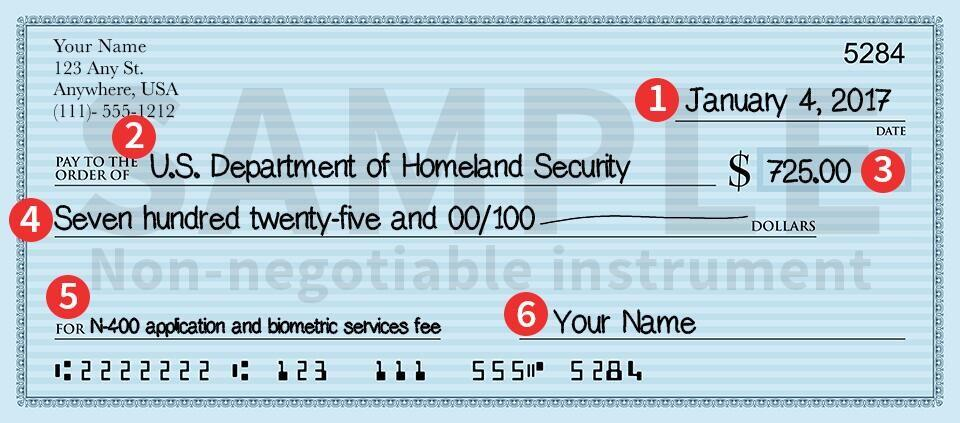
\includegraphics[width=0.8\textwidth]{aux/check.jpeg}
\end{figure}

\vspace*{5em}



\begin{center}
\Large{\textbf{TABLE OF CONTENTS}} 
\end{center}



\begin{enumerate}
 \item Form G-1145 e-Notification of Application/Petition Acceptance
 \item Form I-140, Immigrant Petition for Alien Worker, with \$700 filing fee
 \item Form I-907, Request for Premium Processing Service, with the \$2,500 filing fee
 \item Photocopies of the passport, J-1 visa stamp, three Forms DS-2019 (last three years) and Form I-94
 \item Initial Evidence in Support of the I-140 Immigrant Petition
 \item Statement from Dr. Razvan Marinescu detailing plans on how he intends to continue work in the United States
 \item List of Exhibits
 \item Exhibits 1--25
\end{enumerate}


\pagebreak

% \renewcommand\href[3][\relax]{#3}

% \maketitle

\sloppy

% \section{Introduction}

\vspace{4em}


\begin{center}
 \Large{\textbf{Initial Evidence in Support of the I-140 Immigrant Petition}}
\end{center}

\vspace{4em}


\begin{tabular}{ll}
\textbf{Petitioner and Beneficiary:} & Razvan Marinescu\\
\textbf{Classification Sought:} & Employment-Based Immigration, First Preference\\
& Extraordinary Ability in Science (EB-1A).\\
& Sec. 203(b)(1) INA [8 U.S.C. 1153].\\
\end{tabular}

\vspace{2em}


To whom it may concern,

\vspace{2em}



\newcommand{\fie}{Artificial Intelligence in Medicine}
\newcommand{\dr}{Dr. Marinescu }
\newcommand{\drs}{Dr. Marinescu's }

\newcommand{\qu}[1]{\say{\emph{#1}}}

\newcommand{\pg}{(QR, Professor of EECS, MIT)\\}
\newcommand{\ty}{(UZ, Professor of Electrical and Computer Engineering, Univ A)\\}
\newcommand{\fb}{(GC, Professor of Neuroradiology, University of ABC)\\}
\newcommand{\se}{(TF, Professor of Neuropsychology, XYZ)\\}
\newcommand{\sh}{(TI, Vice President of M, Company XYZ, USA)\\}
\newcommand{\ch}{(DI, Senior Director of XYZ, Company ABC, USA)\\}
\newcommand{\eb}{(FC, Professor at UV)\\}
%\newcommand{\un}[1]{\ul{#1}}





This letter is respectfully submitted in support of the petition of Dr. Razvan Marinescu for classification as a qualified immigrant under the first preference employment immigration for Aliens of Extraordinary Ability pursuant to section 203(b)(1)(A) of the Immigration and Nationality Act (“the Act”). This evidence shows that Dr. Marinescu is an alien of extraordinary ability in the sciences, specifically in \underline{\fie{}}, who sustained national and international acclaim and his achievements have been recognized in the field of expertise. More precisely, this letter provides evidence that:
\begin{enumerate}
 \item \dr satisfies \underline{four} \tc{[three is minimum, but if you can, do an extra one to be on the safe side]} of ten criteria listed in 8
CFR, Section 204.5(h)(3), namely:
\begin{itemize}
 \item Evidence of \drs original scientific and scholarly contributions of major
significance in the field. (section \ref{original})
 \item \drs authorship of scholarly articles in the field in professional media. (section \ref{authorship})
 \item Participation of \dr as a judge of the work of others in the field of
\fie{} (section \ref{reviews})
 \item Evidence that \dr has performed in a critical role for organizations that have a
distinguished reputation. (section \ref{leader})
\end{itemize}
 \item \dr reached a level of expertise indicating that he is one of that small percentage who have risen to the very top of the field of \fie{} -- section \ref{risentotop}.
 \item \dr sustained national or international acclaim and that his achievements have been recognized in the field of \fie{} -- section \ref{sustanedacclaim}.
\end{enumerate}


Pursuant to 8 CFR, Section 204.5(h)(1), \dr may file an I-140 visa petition for classification under Section 203(b)(1)(A) of the Act as an alien of extraordinary ability in the sciences on his own behalf.\\

Pursuant to 8 CFR, Section 204.5(h)(5), neither an offer for employment in the United States nor a labor certification is required for this classification.



\section{Summary of \drs achievements and qualifications}

\dr is a Postdoctoral Researcher in the Computer Science and Artificial Intelligence Laboratory (CSAIL) at the Massachusetts Institute of Technology (MIT) \cite{mitoffer}. \dr joined MIT in February 2019, after finishing his PhD from University College London (UCL). His research focuses on Artificial Intelligence (AI) for Medicine, with a strong focus on neuroscience applications. Before coming to the United States, he has lived in the United Kingdom for 8 years, where he pursued his undergraduate degree at Imperial College London and PhD at University College London, two leading universities worldwide \cite{cv} \cite{degrees}. \dr graduated with First Class Honours in Computer Science at Imperial College London \cite{degrees}.\\

% general: strong background, PhD at UCL, postdoc at MIT, expert in ``medical AI``.
\dr works on Artificial Intelligence (AI) for Medicine, which involves creating state-of-the-art algorithms for understanding, preventing, and solving human diseases, thus enabling the highest quality healthcare for everyone. Artificial Intelligence is predicted to have a tremendous impact in healthcare, from enabling better decision making, to making medical scans and data of much better quality, faster and cheaper. \drs work in particular focuses on creating AI algorithms that perform medical diagnoses with unprecedented accuracy, and as early as possible, and AI algorithms that map the temporal progression of diseases. \dr has worked for more than 6 years on building Artificial Intelligence algorithms for predicting the progression of neurodegenerative diseases such as Alzheimer's disease, currently affecting more than 50 million people worldwide, as well as other neurodegenerative diseases such as Posterior Cortical Atrophy, Multiple Sclerosis and Frontotemporal dementia. \\

%% go through each sub-section and criteria, make a short summary of each

% contributions of major significance to the field
\dr has made contributions of major significance to the field of Artificial Intelligence in Medicine. He performed the first comprehensive study for estimating the progression of Posterior Cortical Atrophy (section \ref{originalpca}), a neurodegenerative syndrome affecting around 2.5 million people worldwide. He also created TADPOLE (section \ref{tadpoleScientific}), the most widely-used challenge and benchmark for algorithms to predict Alzheimer's disease, which had a major impact not just in academia, but also in the biopharmaceutical industry, due to fundamental implications on how Alzheimer's patients are selected for clinical trials. \dr also created DIVE (section \ref{dive}), a computational model that estimates the progression of Alzheimer's disease, for which he was nominated as runner-up for the Francois Erbsmann prize at the International Conference on Information Processing in Medical Imaging (IPMI). \dr also made contributions of major significance on modelling the progression of Multiple Sclerosis and Frontotemporal dementia (section \ref{ms}), having co-authored highly influential articles with more than 100 citations each. \\

% articles published
\dr has authored 25 peer-reviewed scientific articles (12 as first author) that have been published in the top journals in the Artificial Intelligence and medical imaging fields (section \ref{authorship}). The articles \dr authored have gathered more than 485 citations as of June 2021 \cite{gscholar}, and have been cited 154 times in the last 6 months alone, showing an exponential increase in the impact of his work. \drs articles have been published in leading journals and conferences in the field, and have gathered significantly more citations than the articles of his peers (section \ref{articlespeers}). \\

% reviewing work
\dr has also been a judge for the work of others, having been a reviewer on more than 30 scientific articles in 11 leading journals and conferences in the fields of medical Artificial Intelligence and related disciplines (section \ref{reviews}). \\


% performance in leading roles: MIT PDA, 
\dr has been a leader of two distinguished organizations. First, he was the President of the MIT Postdoctoral Association (section \ref{pdaleaderlabel}), representing all postdoctoral researchers at MIT, currently numbering 1400, in matters related to the MIT administration as well as in the planning of career events for postdoctoral researchers. Under \drs leadership, the Postdoctoral Association started advocacy efforts for better housing for postdocs, increased childcare support, and improved career development programs, which impacted all postdoctoral researchers at MIT. As the President of the MIT Postdoctoral Association, \dr was also on the hiring committee of the MIT Institute Community and Equity Officer (ICEO), a key role in the university that reports straight to the provost. Secondly, \dr also organized TADPOLE (section \ref{tadpoleleaderlabel}), currently the leading benchmark worldwide on AI models for predicting Alzheimer's disease. TADPOLE had a significant impact on Alzheimer's disease research, both in academia as well as the biopharmaceutical sector, and brought together a community of thirty-three international teams to create state-of-the-art AI models. \\

As evidenced by seven recommendation letters from distinguished professors within academia and managers in the biotechnology industry, his 25 scientific publications and 30 peer-reviews, as well as his leadership roles, \dr has raised to the very top of the field of medical AI (section \ref{risentotop}). \dr has further sustained this performance, as evidenced by the increasing number of citations obtained recently (154 in the last 6 months alone), and the four invited talks he gave in the last 12 months at prestigious universities in North America: Harvard University, Stanford University, University of British Columbia and University of California Santa Cruz. In addition, \drs research achievements have recently been documented in \emph{Adevarul}, one of the most widely-circulated and trusted newspapers in Romania \cite{adevarul}. 


\section{Proof of \drs Extraordinary Ability}


% !!! 1. Determine whether the alien has made original
% contributions in the field.
% !!! 2. Determine whether the alien’s original contributions are
% of major significance to the field.
%
% You must evaluate whether the original work constitutes major,
% significant contributions to the field. Although funded and
% published work may be “original,” this fact alone is not sufficient % to establish that the work is of major significance. For example, % peer-reviewed presentations at academic symposia or peer reviewed articles in scholarly journals that have provoked widespread commentary or received notice from others working in the field, or entries (particularly a goodly number) in a citation index which cite the alien's work as authoritative in the field, may be probative of the significance of the alien’s contributions to the field of endeavor. 

\subsection{Evidence of original scientific, scholarly, artistic, athletic, or business-related contributions of major significance to the field}
\label{original}


% PCA
\subsubsection{Evidence of original scientific contribution: First comprehensive study estimating the progression of Posterior Cortical Atrophy}
\label{originalpca}

\dr performed the first comprehensive study for estimating the progression of Posterior Cortical Atrophy, a neurodegenerative disease that affects the posterior part of the brain. While previous studies have only qualitatively analysed isolated case reports, \dr analysed the first comprehensive population of 102 patients with Posterior Cortical Atrophy, and was the first to run computational models to map the progression of the disease over time. The article, published in the journal Brain in 2019, has already been cited 37 times as of June 2021 \cite{pca}. \\

\qu{% PCA
Dr. Marinescu has further made landmark contributions to the study of Posterior Cortical Atrophy, a variant of Alzheimer's disease that affects the visual cortex. Compared to typical Alzheimer's disease, the progression of Posterior Cortical Atrophy was until recently poorly understood. Dr. Marinescu, through his scientific article published in the journal Brain as well as his PhD thesis, \ul{elucidated the temporal progression of Posterior Cortical Atrophy, and showed that it is indeed distinct from that of Alzheimer's disease}. He further analysed the progression patterns in three different subgroups of Posterior Cortical Atrophy with different clinical presentations, and showed that these subgroups again have different progression profiles of brain atrophy. \ul{These contributions are fundamental for clinical trials in Posterior Cortical Atrophy}, and will help the management of all patients suffering from Posterior Cortical Atrophy, currently believed to number approximately 2.5 million people worldwide.} \fb

\qu{Dr. Marinescu, in collaboration with Dr. Firth and Dr. Primativo, authored the first comprehensive longitudinal study on the progression of Posterior Cortical Atrophy. In this landmark study, Dr. Marinescu used Artificial Intelligence models to estimate the evolution of brain atrophy in the largest study population of subjects of Posterior Cortical Atrophy to date. He elucidated precisely which brain regions are affected, and in which exact temporal order, which was until then poorly understood. The article, while recently published in 2019, has already been cited more than 32 times. \ul{As a leading expert in Posterior Cortical Atrophy, I can certify that this study was of paramount importance for the field}: it provided the very first glimpse into the temporal evolution of Posterior Cortical Atrophy, which is necessary for understanding its fundamental mechanisms and for running future clinical trials. In addition, given that most subjects with Posterior Cortical Atrophy are given drug treatments normally given for typical Alzheimer's disease, \ul{this study provided strong evidence that Posterior Cortical Atrophy is likely to be a different disease that will require specialised drug treatments} compared to typical Alzheimer's disease.} \se

In addition, in his PhD thesis, Dr. Marinescu has also extensively studied the evolution of subgroups of patients with Posterior Cortical Atrophy, the first such study of this kind \cite{pca}. \\
\qu{In his PhD thesis, as well as the article submitted to the Alzheimer's Association International Conference (AAIC), Dr. Marinescu was \ul{among the very first to study the evolution of brain pathology in different subgroups within Posterior Cortical Atrophy}. The work done by Dr. Marinescu proved that different clinical symptoms indeed correspond to different brain regions affected. This work is of major importance for future personalized medicine, as drugs and therapies tailored to specific individuals or subgroups will be more effective and have fewer side effects. } \se

% TADPOLE (as a study)
\subsubsection{Evidence of original scientific contribution: Created the most widely-used challenge and benchmark for algorithms to predict Alzheimer's disease}
\label{tadpoleScientific}

\dr has created ``The Alzheimer's Disease Prediction Of Longitudinal Evolution'' (TADPOLE) Challenge, where 33 international teams from both academia and industry built state-of-the-art algorithms to predict the evolution of Alzheimer's disease. \dr not only organised challenge, but also evaluated all submissions from all teams, analysed the final results, and presented them in three scientific articles \cite{tadpole}, as well as at the most prestigious international conferences. This work was of major significance and impact in the research community, as can be seen by the 79 citations obtained by the three TADPOLE articles so far \cite{tadpole}.\\ 

\qu{Dr. Marinescu also ran and analyzed the results of TADPOLE Challenge, an international competition that evaluated algorithms for predicting the progression of individuals at risk of Alzheimer's disease. While previous research algorithms were all tested on different datasets or subsets of the data, this made their comparison extremely difficult. Under Dr. Marinescu's leadership, an entire research community was brought together to focus on a single task. In addition, \ul{the study was extremely unique, because it was completely blind to the evaluation data}, which did not exist at the time the predictions were made as it was acquired afterwards. This made the TADPOLE study completely unbiased, and the only one in our research community to be entirely prospective.} \pg

In addition, \drs TADPOLE work has been recognized by many prominent researchers who have not directly collaborated with him. 

\qu{I have never met Dr. Marinescu in person, but I am aware of his original scientific contributions to the field of medical artificial intelligence. I have first come in contact with his work in 2017, when my research team decided to participate in TADPOLE, the international challenge Dr. Marinescu organized which aimed to evaluate algorithms that predict the progression of Alzheimer's disease. \ul{TADPOLE is a one-of-a-kind challenge and benchmark for comparing a variety of algorithms and methods for the challenging task of predicting Alzheimer's disease}, a key neurodegenerative disease affecting millions of people worldwide. While previous algorithms in our research field were all tested on different datasets and with different target variables to be predicted, \ul{TADPOLE created a standardized evaluation framework which made all algorithms' performance comparable}. Thirty-three international teams from nine different countries, with approximately three members each, participated in the challenge, and submitted a total of ninety-two prediction algorithms.} \ty

The impact of TADPOLE has been significant and can potentially impact millions of patients with Alzheimer's disease worldwide, and helped identify what are the best AI prediction methods in the field:

\qu{Through TADPOLE, Dr. Marinescu made a huge scientific contribution to our research field. First, it helped establish \ul{how well and how early} we can predict Alzheimer's disease with computational algorithms, what are the state-of-the-art algorithms for Alzheimer's disease prediction, and what types of input data are most informative for such predictions. Secondly, Alzheimer's disease is a devastating disease worldwide, with currently more than 50 million people affected, and having associated costs of approximately \$100 billion in the United States alone. \ul{The ability to detect the disease early, using such AI algorithms}, can improve the healthcare management of millions of people worldwide, and also lower the economic costs and caregiver efforts for managing Alzheimer's disease patients.} \ty
\qu{In addition, the contribution of TADPOLE towards the field was immense. In particular, the most surprising result was that while the models could predict the clinical diagnosis and measures from Magnetic Resonance Imaging, they could not reliably predict cognitive scores that are routinely used in clinical trials of Alzheimer's disease. This finding has important implications for clinical trials, and also highly impacted the field: \ul{many researchers are now working on improving the predictions models for cognitive tests.}} \fb
\qu{The impact of the TADPOLE competition in Alzheimer's disease prediction research cannot be overstated: around 30-40 international teams participated in the competition from both academia and the biotech. industry, and \ul{it entirely reshaped the field regarding what are the best AI methods for predicting such a disease.}} \ch

%TADPOLE engagement involved several stakeholders, including international teams, three Alzheimer's disease charities, and was featured in the media\cite{tadpolemedia}.

\qu{The challenge \ul{received a lot of interest from researchers, media and institutions around the world}: more than 30 international teams participated with almost 100 different prediction models, it was featured in the media, and received sponsorship from the three main Alzheimer's disease charities Alzheimer's Association, The Alzheimer's Society, and Alzheimer's Research UK. } \fb

TADPOLE had a major influence not just within academia, but also in the pharmaceutical industry. XX, a major biopharmaceutical company, participated in the challenge, while YY, another major biopharmaceutical company, has closely followed the work: 

\qu{I have first heard of Dr. Marinescu's work in 2017, when \ul{our team at XX decided to participate in the TADPOLE Challenge}, which he organised during his PhD at University College London. As part of the challenge, we had to create an algorithm that could automatically predict which subjects would develop Alzheimer's disease in the future. \ul{This task was well aligned with our objectives} of building computational AI models for early diagnosis of diseases such as Alzheimer's disease. While we had many years of experience with such algorithms, it was not an easy task due to the unfamiliarity with the data. Eventually, we managed to create a good algorithm for making accurate predictions [...].} \ch
\qu{Another influential work by Dr. Marinescu that we have been paying very close attention is the TADPOLE Competition, which compares algorithms at predicting the progression of individuals at risk of Alzheimer's disease. These algorithms are highly useful towards identifying the most suitable patients that can go into our clinical trials, i.e. those that will benefit the most from the drug treatments. \ul{This solves one key issue we often face in clinical trials}, that of cohort diversity due to different underlying genetics and pathology, which often obscures treatment effects. \ul{The computational models from the TADPOLE Challenge can help us select homogeneous groups of patients}, thereby increasing the treatment effects in drug trials.} \sh

The results of TADPOLE have also been featured in the media, such as the article from Alzforum \cite{tadpole}. Alzforum is a website founded in 1996 that brings together a team of specialists in science writing, and presents to the wider public the latest research on Alzheimer's disease \cite{tadpole}.\\ 
\qu{Results are in for the TADPOLE Challenge -- a prize contest that invited researchers to come up with their own ways of predicting dementia symptoms in participants enrolled in the Alzheimer's Disease Neuroimaging Initiative (ADNI). In a live webinar on June 14, organizers announced who came out ahead. Contestants had submitted computer code to forecast the clinical status, cognitive scores, and/or imaging characteristics of ADNI3 participants. Once submissions were in, the data were collected and results tabulated. The best methods garnered prize money in the amount of £30,000, donated by the Alzheimer’s Society in London, Alzheimer’s Research U.K., and the Alzheimer’s Association.} (Gwyneth Dickey Zakaib, Alzforum, 19 Jun 2019)


% Disease progression modelling: DIVE, DKT
\subsubsection{Evidence of original scientific contribution: Created DIVE, a computational model estimating the progression of Alzheimer's disease}
\label{dive}

\dr has also published ``Data-driven Inference of Vertexwise Evolution'' (DIVE), a model for estimating the progression of brain pathology in Alzheimer's disease. His work was nominated as runner-up for the Francois Erbsmann prize at the Information Processing in Medical Imaging (IPMI) conference. The Francois Erbsmann prize is a prize given to one person every year, for outstanding contributions to the field, and is the only prize awarded by the IPMI conference. 

\qu{In his pioneering work at the IPMI conference, he [Dr. Marinescu] proposed DIVE, a model for predicting the progression of Alzheimer's disease at each location on the brain. While previous progression models used a very simplistic assumption of averaging measurements of brain pathology across entire brain regions, this did not allow one to see fine-grained patterns of pathology that affect small regions in the brain. As an analogy, imagine a world map showing the population density in each country. While that is very informative in itself, it cannot give information about the variation of density within a particular country. \ul{Dr. Marinescu's contribution, translated to this world map, enabled one to measure the population density at the resolution of small cities and towns}, and in addition, also measure population trends over time. However, solving this problem for the human brain was extremely difficult computationally and mathematically due to the fact that there are more than 100,000 3D pixels in a single brain image, and such a study required thousands of images to be analyzed together. \ul{To overcome these fundamental limitations, his insight was to use techniques from unsupervised learning to cluster trajectories based on their similarity.} This creative solution opened up the possibility of studying brain diseases at a much better resolution than previously possible, and allowed neuroscientists to significantly improve their understanding of mechanisms underpinning brain diseases.} \pg

The DIVE model had a substantial impact in the field. The two articles \cite{dive} published by \dr in prestigious publication venues, were cited more than 44 times as of June 2021 and resulted in further developments by research groups around the world.\\
\qu{The DIVE model was a highly original contribution to the field and was very well-received at the Information Processing for Medical Imaging conference (IPMI), having been nominated for the Francois Erbsmann prize. As an expert in the field, I can attest that IPMI is one of the leading venues in medical image analysis and medical artificial intelligence, and only outstanding contributions are considered for the Francois Erbsmann prize at IPMI. The paper has since gathered 23 citations, and \ul{a follow-up model that builds on DIVE has already been implemented by the research team at INRIA, France}. In addition, Dr. Marinescu's DIVE article was published in the NeuroImage journal. As the editor of the journal myself, I can confirm that the \ul{acceptance standards are very high}, with only the best articles being accepted for publication.} \ty
\qu{The DIVE model can be used not only to predict the future evolution of Alzheimer's disease subjects, but also to identify new Alzheimer's disease biomarkers that can be used to diagnose the disease and monitor its progression. My team at XX has been working for several years on developing novel biomarkers of Alzheimer's disease, and \ul{I can confirm that Dr. Marinescu's work is of fundamental importance for the research field}, and had a significant impact on future development of AI prediction models for Alzheimer's disease. It was for instance cited more than 24 times, while the precursor to DIVE, also by Dr. Marinescu[2], was cited more than 14 times so far.} \ch


\subsubsection{Evidence of original scientific contribution: Disease progression modelling of Multiple Sclerosis and Frontotemporal dementia}
\label{ms}

% MS

\dr co-authored a number of influential publications which used computational models to study Multiple Sclerosis and Frontotemporal dementia, two devastating neurodegenerative diseases affecting several million people worldwide. For Multiple Sclerosis, Dr. Marinescu, in collaboration with Dr. Eshaghi, authored the largest study \cite{dpm} to date on the progression of Multiple Sclerosis,  which revealed that the brain pathology spreads in a particular sequence that they closely described. This publication received more than 106 citations to date, and represents a landmark study in the field. \\ %In another publication \cite{dpm} co-authored by \dr, the progression of Multiple Sclerosis was characterised in relation to known neural connections between different brain region, the first such study in the literature. Although this article was just published December 2020, it was already cited 5 times. \\
\qu{In another landmark study Dr. Marinescu co-authored with Dr. Eshaghi, they applied such disease progression models on the largest cohort to date of subjects with Multiple Sclerosis, and \ul{found that the brain gray matter is affected in a specific sequence of events that they described}. The publications are both well cited, and their models widely used in the research community, with [...] the Multiple Sclerosis study already receiving more than 104 citations. As one of the world experts in Multiple Sclerosis and Alzheimer's disease, I can confirm that \ul{such models are of crucial importance for identifying the right subjects for clinical trials}, and I am aware that \ul{pharmaceutical companies are already using their models for the analysis of their imaging data} in Alzheimer's disease and Multiple Sclerosis drug trials.} \fb
\qu{Dr. Marinescu, together with Dr. Eshaghi, also authored a prominent study on the evolution of Multiple Sclerosis in \ul{the largest cohort to date} (more than 3000 subjects), which demonstrated that the \ul{brain regions in Multiple Sclerosis become affected in a precise sequence that they mapped}. Dr. Marinescu has also recently co-authored another study in the Elife journal on the role that brain neural connections play in Multiple Sclerosis and Alzheimer's disease, as well as another publication on the progression of Huntington’s disease, a neurodegenerative disease affecting the motor cortex. \ul{All these publications highlight the wide remit of Dr. Marinescu's AI models, in particular the disease progression models}, that can be applied to many different brain diseases in order to clarify and understand their progression over time. Given the millions of people around the world affected by these diseases, Dr. Marinescu’s work is of large impact to society.} \se

In addition, \drs modelling approach was adopted by XYZ, a large pharmaceutical company, for their Multiple Sclerosis clinical trials. This highlights the impact this work had not just within academia, but also in the biopharmaceutical industry.\\
\qu{... Dr. Marinescu has also co-authored another high-profile article on mapping the evolution of neurodegeneration in Multiple Sclerosis using disease progression models. We at XX have been extremely interested in the modelling approach used by Dr. Marinescu, and \ul{have used it for our brain imaging data in Multiple Sclerosis}. I should highlight that such models are critical for our 5 clinical trials in Alzheimer's disease, as well as our 2 clinical trials in Multiple Sclerosis, as they can predict the disease evolution of individual subjects undergoing the clinical trials, help select the most suitable subjects for going into the trial, and help select the right target measure for evaluating the drug effects. \ul{Given the potential to impact all our clinical trials}, that incur costs in the order of millions of dollars, our \ul{Artificial Intelligence team has implemented and built on Dr. Marinescu's models.}} \sh
%\qu{Dr. Marinescu's work on understanding disease progression of Alzheimer's disease and Multiple Sclerosis can have immense implications for clinical trials. Both diseases affect millions of people worldwide, and have devastating effects on their cognition. In addition, there are currently no treatments for Alzheimer's disease that can stop cognitive decline, and all clinical trials so far have failed due to wrong treatment targets, wrong patients selected for trials, and difficulty in measuring treatment effects. Through Dr. Marinescu's work, which improves the understanding of such diseases, and could lead to better targets and cohort selection, there is increased hope that working treatments for Alzheimer's disease will be found in the future.} \sh %NOT USED ANYWHERE SO FAR


% FTD
Dr. Marinescu, alongside Dr. Young, has also authored the Subtype and Stage Inference, a novel computational model that revealed previously unknown variability in Frontotemporal dementia, a brain disease that affects the frontal and temporal lobes.  This study \cite{dpm}, published in Nature Communications, has been of major impact in the field, having been cited 101 times as of June 2021.     \\
\qu{Dr. Marinescu has also authored other prominent works on disease progression models. The "SuStaIn" model, published in the Nature Communications journal, is a novel technique that can find, within a disease population, multiple sub-populations that progress with different disease patterns. \ul{The SuStaIn model discovered that, in Frontotemporal Dementia, the patients with a specific mutation (C9orf72) were actually composed of two distinct groups, instead of a single uniform group as it was believed until that time.}} \ty
\qu{Dr. Marinescu has done outstanding work on brain diseases other than Alzheimer’s [disease] and Posterior Cortical Atrophy. \ul{His seminal work on the Subtype and Stage Inference (SuStaIn) model has revealed the precise variability in brain pathology in patients with Frontotemporal dementia (FTD), and importantly, found that the patients with the C9orf72 mutation are more diverse than previously thought.} } \se

% Dr. Marinescu's disease progression modelling work, including the SuStaIn model, has also attracted the attention of XX, who invited him to present his results. \\
% \qu{I first met Dr. Marinescu in October 2020, when XYZ, the Director of Artificial Intelligence at XX, invited Dr. Marinescu to present and discuss his work on disease progression modelling. Dr. Marinescu co-authored a highly influential article on a novel disease progression model called SuStaIn, that can identify, within a specific disease, multiple subgroups with different progression profiles.} \sh

Finally, this line of work, as emphasized by Dr. XX, can have tremendous impact on US healthcare, given that millions of people are affected by Alzheimer's disease and the lack of suitable treatments.\\
\qu{Dr. Marinescu is also very well-known for his work on disease progression models, a specific class of medical AI models which predict not just the diagnosis of a particular patient, but their entire future progression. He worked on several major research projects in this line of research, such as a key study of Multiple Sclerosis, which gathered more than 106 citations so far, and the SuStaIn model, which gathered more than 85 citations so far, and characterised the disease variability in both Alzheimer's disease and Frontotemporal Dementia. \ul{Given the huge burden of such diseases, affecting more than 3 million people just in the United States alone, and the lack of suitable treatments, the work of Dr. Marinescu is of paramount importance for healthcare in the US and worldwide}, and can have even more impact in the future.} \ch



% !!!! 1. Determine whether the alien has authored scholarly
% articles in the field.
% As defined in the academic arena, a scholarly article reports on
% original research, experimentation, or philosophical discourse. It
% is written by a researcher or expert in the field who is often
% affiliated with a college, university, or research institution. It
% should have footnotes, endnotes, or a bibliography, and may
% include graphs, charts, videos, or pictures as illustrations of the
% concepts expressed in the article.
% !!!! 2. Determine whether the publication qualifies as a
% professional publication or major trade publication or a
% major media publication. 

\subsection{Evidence of authorship of scholarly articles in professional or major trade publications or other major media}
\label{authorship}

\subsubsection{\dr has published 25 scientific articles in the field of Medical Artificial Intelligence}

% All articles: how many, citations, publication venues, impact factor, downloads, 
As evidenced in \drs Curriculum Vitae \cite{cv} and in his Google Scholar profile \cite{gscholar}, \dr has so far authored more than 25 scientific articles (12 as first author), which have together gathered more than 485 citations \cite{gscholar} as of April 2021. Three of the papers he authored have received more than 20 citations in 2020 alone, comparable to top 100 papers in the field of medical artificial intelligence \cite{nadri2017top}. \\

The most important of \drs publications, alongside their impact in the field, have been presented in detail in section \ref{original} and are shown in \cite{pca}, \cite{tadpole}, \cite{dive} and \cite{dpm}. Other important publications not described there also include Disease Knowledge Transfer, an AI model that can transfer information from common neurodegenerative diseases such as Alzheimer's disease to rarer diseases such as Posterior Cortical Atrophy \cite{otherpub}. BrainPainter, an article authored by \dr introducing a software to visualize brain images, has already been cited 14 times since it's publication in November 2019 \cite{otherpub}. With collaborators Dr. Alexandra Young and Dr. Peter Wijeratne at University College London, \dr co-authored novel disease progression models for Alzheimer's disease as well as Huntington's disease, which have each been cited more than 23 times since their publication \cite{otherpub}. In addition, \drs PhD thesis contains work on 5 research directions that have been published in more than 7 research articles at journals and conferences in the field \cite{pca}.  


\subsubsection{\drs publications have been published in the leading journals and conferences in his field}

\drs scientific articles have been published in the leading venues in Artificial Intelligence and Medicine, which include:
\begin{itemize}
    \item Brain: top neuroscience and neurology journal, with impact factor of 11.3, has been in circulation since 1878. \dr authored two articles in Brain \cite{cv}.
    \item Nature Communications: leading journal with a wide life-science remit, impact factor of 12.1. \dr authored one article in Nature Communications \cite{cv}.
    \item NeuroImage: the top journal for neuroimaging studies, with impact factor of 5.9. \dr authored one article in NeuroImage \cite{cv}.
    \item Information Processing in Medical Imaging (IPMI): major conference on medical imaging, also the oldest, having first been organised in 1969. \dr authored one article in IPMI \cite{cv}.    
    \item Medical Image Computing and Computer Assisted Surgery (MICCAI): Largest venue in Artificial Intelligence for Medicine, with more than 1,700 delegates and 540 research articles presented in 2019. It is ranked \#1 in the Medical Informatics category \cite{confrankings}. \dr authored four articles in MICCAI and its workshops \cite{cv}.
    \item Alzheimer's Association International Conference: the largest conference on Alzheimer's disease, with audience ranging from researchers in fundamental science, biopharmaceutical companies, and clinical practitioners. \dr authored four articles in the AAIC conference \cite{cv}.
\end{itemize}

Dr. XX and Prof. XX have also confirmed that \drs work is published in the leading international venues, which have a very high standard for accepted articles.\\

\qu{As an expert in the field, I can attest that \ul{Dr. Marinescu published in the leading journals and conferences in medical AI as well as neurology}. The Medical Image Computing and Computer Assisted Surgery (MICCAI) conference, where Dr. Marinescu authored three papers, is the leading venue on theoretical and technical work on artificial intelligence and machine learning for medical applications, having an impact factor of 11.14. On the other hand, the neurology journal "Brain", where Dr. Marinescu authored two articles, one as joint-first author and the other as second author, is the one of the leading journals on neurology and neuroscience, which has been circulating since 1878 and has an impact factor of 11.33.}\ty

\qu{\ul{Dr. Marinescu authored articles in the leading journals and conferences of the field}. Nature Communications, where Dr. Marinescu co-authored the SuStaIn model, is a journal of outstanding research in all areas of natural sciences, with a 2-year impact factor of 12.121. Brain is one of the leading journals on neuroscience and neurology, where Dr. Marinescu published two articles, one as joint-first author. Neuroimage is another leading journal covering research in neuroimaging, with an impact factor of 5.8. Several well-known and prolific authors have published in Neuroimage, including Karl Friston and Arthur W. Toga. In terms of conferences, Dr. Marinescu has published multiple articles in the Medical Image Computing and Computer Assisted Interventions (MICCAI) and Information Processing in Medical Imaging (IPMI) conferences. These are highly technical conferences where key AI experts in medicine, as well as AI and pharmaceutical companies attend. \ul{As a clinical researcher in brain diseases, I can confirm that many of the methods published in these two conferences have a strong downstream impact on the medical problems we work on.}} \se

\subsubsection{\drs scientific articles have been cited significantly more than the articles of his peers}
\label{articlespeers}

The articles authored by Dr. Marinescu have been cited significantly more than the average of their field, as compared to the impact factor of the journals and conferences where they were published (the impact factor measures how many citations an article from that respective journal receives on average in the 2 years since its publication). \drs articles published in the Brain journal have gathered 54 and 32 citations within the first two years, significantly higher than the average of 11.3 citations articles in the Brain journal gather in their first two years. Similarly, \drs Nature Communications article gathered 59 citations in the first 2-years, significantly higher than the average of 12.1 citations for articles in that journal, while his NeuroImage article gathered 24 citations, significantly higher than the average of 5.9 citations for articles in that journal.\\

When taking all publications of \dr into account, his 485 citations gathered so far place him within the top 1\% percentile of scholars in Computer Science according to the ESI ranking \cite{esi}.
%TODO: add also the ESI and G Scholar rankings here.


%\subsubsection{\drs scientific articles have been featured in published media}

%
%Two of the articles \dr published \cite{tadpole}, which focused on the design and results of the TADPOLE competition and benchmark for Alzheimer's disease prediction, have been featured in media articles, such as two articles from Alzforum\cite{tadpolemedia}, the largest media organization covering Alzheimer's disease research worldwide.

% No UCSIS guidance 

\subsection{Evidence that \dr has been asked to judge the work of others in medical Artificial Intelligence and adjacent areas}
\label{reviews}

% All Reviews
\dr has been a reviewer on multiple years for the top conferences and journals in the fields of artificial intelligence, machine learning, computer vision, and medical imaging \cite{reviews}:
\begin{itemize}
    \item Computer Vision and Pattern Recognition (CVPR): with an impact factor of 51.9 and an h5-index of 299, it is ranked \#1 by guide2research.com among Machine Learning and Artificial Intelligence conferences  \cite{confrankings}.
    \item Neural Information Processing Systems (NeurIPS): with an impact factor of 39.4 and an h5-index of 198, it is ranked \#2 by guide2research.com among Machine Learning and Artificial Intelligence conferences \cite{confrankings}.
    \item International Conference on Machine Learning (ICML): with an impact score of 18.4 and an h5-index of 171, it is ranked \#6 in Artificial Intelligence and Machine Learning \cite{confrankings}. 
    \item Medical Image Computing and Computer Assisted Surgery (MICCAI): with an impact factor of 9.7 and an h5-index of 61, it is ranked \#1 by guide2research.com in Biomedical and Medical Informatics.
    \item Information Processing in Medical Imaging (IPMI): with an impact score of 3.13, IPMI is widely recognized as a preeminent international forum for presentation of cutting edge research in the medical imaging field. \cite{confrankings}
    \item NeuroImage: with an impact factor of 5.88 and an h5-index of 115, NeuroImage is the most selective journal for neuroimaging analysis. \cite{confrankings}
    \item Nature Communications: with an impact factor of 12.1, it is a leading journal in the natural sciences. \cite{confrankings}
    \item Medical Image Analysis (MedIA): with an impact factor of 11.1 and an h5-index of 67, it is a leading journal in medical imaging research. \cite{confrankings}
    \item IEEE Transactions on Pattern Analysis and Machine Intelligence (PAMI): with an impact factor of 17.8 and an h5-index of 131, it is a leading computer vision journal \cite{confrankings}.
%     \item Alzheimer's and Dementia: with an impact factor of 17.12 and an h-index of 94, Alzheimer's and Dementia is the leading journal worldwide on Alzheimer's disease research, and is supported and funded by Alzheimer's Association, the largest Alzheimer's disease organization worldwide. \cite{confrankings}
    \item Journal of Alzheimer's Disease (JAD): with an impact factor of 3.9, JAD is a well-known journal focusing on etiology, pathogenesis, epidemiology, genetics, treatment, and psychology of Alzheimer's disease.  
\end{itemize}

\dr has reviewed a total of 30 scientific articles \cite{reviews}: 1 article for CVPR, 3 for NeurIPS, 6 for ICML, 6 for MICCAI, 8 for IPMI, 1 for NeuroImage, 1 for Nature Communications, 1 for MedIA, 1 for PAMI and 2 for JAD. While \dr has reviewed significantly for conferences in the field of medical Artificial Intelligence, Computer Vision and adjacent areas, this is because in these fast-moving fields, most researchers do not publish in journals. In addition, these conference publications are not just abstracts, but full scientific articles of at least 8-10 pages, with consistent supplementary material, and provide significant theoretical and experimental advances on the explored topic. \\

\qu{\ul{The journals and conferences Dr. Marinescu has published and reviewed for are the leading journals in the field}. For example, the journal Brain, on which I serve as an editor, has a very high acceptance standard, and only the leading scientific articles with major impact to the field are accepted. Other journals such as Nature Communications and NeuroImage also have a similarly high standard. Similarly, the leading international conferences in medical AI, Medical Image Computing and Computer Assisted Intervention (MICCAI) and Information Processing in Medical Imaging (IPMI), also only accept truly novel contributions. In addition, in contrast to conferences that only require abstract submissions, these conferences require articles fully describing the methods and results in their entirety, so publications in MICCAI and IPMI are often comparable to journal publications in their own right. } \fb

\qu{Dr. Marinescu has not only published in the leading journals and conferences of the field, but also reviewed the work of other scientists for these journals. \ul{This is a crucial service for the research community, as it helps keep the publication standard to a very high quality. I should emphasize that only leading researchers with domain knowledge and expertise are invited to review for such journals and conferences.}} \se

% !!! 1. Determine whether the alien has performed in leading or
% critical roles for organizations or establishments.
% In evaluating such evidence, you must examine the role the
% alien was hired or appointed to fill for the organization or
% establishment and determine whether that role is (or was)
% “leading” or “critical.” The evidence must establish that the
% alien has been a leader or has somehow contributed in a way
% that is of significant importance to the outcome of the
% organization or establishment’s activities. A supporting role
% may be considered “critical” if the alien’s performance in the
% role is (or was) important in that way. It is not the title of the alien’s role, but rather the alien’s performance in the role that determines whether the role is leading or critical. In addition, a key question may be whether the alien's role was leading or critical to the organization as a whole.
% 
% !!! 2. Determine whether the organization or establishment
% has a distinguished reputation.
% Keep in mind that the relative size or longevity of an
% organization or establishment is not in and of itself a
% determining factor. Rather, the organization or establishment
% must be recognized as having a distinguished reputation.
% Webster’s online dictionary defines distinguished as 1: marked
% by eminence, distinction, or excellence <distinguished
% leadership and 2: befitting an eminent person <a distinguished
% setting. 


% wegreened advice: add at least 2 different leading roles. The requirement uses plurality (leading role``S'')


\subsection{Evidence of \drs performance in a leading role in distinguished organizations}
\label{leader}


\subsubsection{\dr was the President of the MIT Postdoctoral Association}
\label{pdaleaderlabel}

\paragraph{The MIT Postdoctoral Association is a distinguished organization}\mbox{}\\

% 6990 graduate students - https://web.mit.edu/facts/enrollment.html
% 6000 grad students - https://gradadmissions.mit.edu/about
% 1400 postdocs - http://web.mit.edu/fnl/volume/262/sive_etal.html
% faculty: 1,067 (excl. teaching faculty) http://web.mit.edu/facts/faculty.html
% research staff: 1766 http://web.mit.edu/facts/faculty.html
% postdocs / all ~ 13% of research population

% MIT is a distinguished organization + 
The Massachusetts Institute of Technology is the world's leading institute in modern science, engineering, mathematics and technology, and ranks among the most prestigious academic institutions in the world. MIT employs approximately 11,000 research staff: 6990 graduate students, 1400 postdoctoral researchers, 1067 faculty and 1766 research staff \cite{pdaleader}. \\ 

% Postdoctoral Researchers are a critical group of the MIT research community
The postdoctoral researchers, comprising approximately 13\% of the researchers at MIT, are critical for the research environment at MIT: given their completion of the PhD and dissertation, they have ample expertise in a given topic which they pass on to the junior researchers, and further deepen or broaden their dissertation research. In addition, they often supervise graduate students and lead research projects in the laboratory.\\

% PDA, what is the PDA
The MIT Postdoctoral Association (PDA) is an MIT-wide organization which runs career and personal development programs for all Postdoctoral Researchers at MIT, currently numbering more than 1,400. Furthermore, it works with the MIT administration to enhance and improve all aspects of the postdoctoral research experience. \ul{Given it is the only organization that represents all postdoctoral researchers at MIT, it's role is critical for all the 1400+ postdoctoral researchers at MIT and for the entire MIT research community.}  \\
\qu{The MIT Postdoctoral Association (PDA) is an organization that supports MIT postdoctoral researchers during their professional research and career development. The Association oversees all postdoctoral researchers at MIT, currently numbering more than 1500, which are spread across more than 50 research centers and institutes across MIT. The association serves as a liaison between postdoctoral researchers and the faculty and administration of MIT, and strives to engage with and improve the MIT community. The MIT PDA aims to enhance all aspects of the postdoctoral research experience, and foster a sense of community which promotes and encourages an environment of peer support. The MIT PDA has an Executive Board which is responsible for the general operations, and is currently composed of five executive officers: President, Vice President, Treasurer, Corresponding Secretary and Recording Secretary. The association also comprises a standing committee of around nine additional officers, responsible for fulfilling specific responsibilities. The MIT PDA is governed by a constitution, which was last ratified in 2012. \ul{Given all the functions and responsibilities that the Postdoctoral Association has, its role is of critical importance for all postdoctoral researchers at MIT, and for MIT altogether.}  } \eb

\paragraph{As the President of the MIT Postdoctoral Association, \dr was in the leading role}\mbox{}\\

% PDA President role
The PDA President position is highly competitive and is obtained through an electoral process where all postdoctoral researchers at MIT vote on multiple candidates based on their manifesto and prior leadership experience. \dr was elected due to his his sound manifesto outlining several key proposals that will improve the MIT postdoctoral experience, alongside prior leadership experience at Imperial College and University College London. \cite{pdaleader} \\
\qu{Dr. Marinescu was initially elected in August 2019 as Vice President of the PDA by the MIT postdoctoral researchers. However, two months later, due to the previous President having to unexpectedly leave the role, Dr. Marinescu was voted by the PDA board as the new President. [...] I should emphasize that \ul{obtaining such an executive role in the Postdoctoral Association is extremely difficult}, as anyone of the 1500 postdoctoral researchers at MIT can stand for election, and \ul{the candidates each need to prepare a clear manifesto outlining solutions to key problems}, and convince all other postdoctoral researchers to vote them. Prior leadership experience is also essential to be elected in such a role.} \eb

The PDA President role that \dr had comes with significant responsibilities, such as presiding and chairing the General Board Meetings of the Postdoctoral Association, representing the association in the meetings with the MIT administration, and internally, running the association and training all incoming officers.\\
\qu{In the role of PDA president, Dr. Marinescu had significant responsibilities. He presided, chaired and set the agenda for all General Meetings, acted as a liaison between the MIT PDA and the Office of the Vice President for Research, acted as a representative of MIT PDA in the Faculty Postdoc Advisory Committee. Internally, he was responsible for the overall condition of the Postdoctoral Association, ensured that all other officer positions are filled, and coordinated the training of incoming officers. The \ul{PDA President role is very demanding, as it involves organizing and running a board of 15-20 PDA officers}, representing all MIT postdoctoral researchers, currently numbering more than 1500, in faculty meetings and externally outside MIT, and \ul{listening to the needs of postdoctoral researchers and working with the PDA board to find solutions.}} \eb




% Impact
\paragraph{\drs leadership in the MIT Postdoctoral Association had substantial impact for all postdoctoral researchers at MIT}\mbox{}\\

% Impact of Dr. Marinescu's leadership in the PDA
\dr led the MIT Postdoctoral Association to launch several initiatives, such as career development programs, academic and industry panels, a new Diversity, Equity and Inclusion journal club. In addition, \dr initiated a session for postdoctoral researchers to meet representatives of the MIT Corporation as well as Prof. Maria Zuber, the MIT Vice President for Research. \\
\qu{Under the leadership of Dr. Marinescu, the MIT Postdoctoral Association has had many accomplishments and launched many initiatives for all postdoctoral researchers at MIT. It ran several career development programs, such as a six-month mentorship program for both academia as well as industry, several panel discussions on topics regarding academic research and future career pathways, and also launched a new Diversity, Equity and Inclusion journal club, where MIT postdoctoral researchers discussed scientific articles on diversity and inclusion topics. They also started collaborations with other Postdoctoral Associations, such as the Boston-Area PDA, as well as the Harvard PDA. \ul{Perhaps one of the most important initiatives undertaken by Dr. Marinescu was to organize a session where 10 representative postdoctoral researchers across MIT met with 15 members of the MIT Corporation who were visiting the office of the Vice President for Research}, in order to give them feedback about postdoctoral academic life. The session had a \ul{major impact for all postdoctoral researchers at MIT}, as it provided the required impetus to address multiple problems, in particular regarding housing affordability and general living expenses.} \eb

\dr also led advocacy efforts in new directions, such as for better housing and child support for postdoctoral researchers with families: \\
\qu{Dr. Marinescu, as PDA President, has also led new directions of advocacy for the PDA. \ul{During his tenure, the PDA has started advocating on key issues facing postdoctoral researchers at MIT}: the ability to find affordable housing, increased childcare support for researchers with children, improved career development programs, and more opportunities for interaction and collaboration between postdoctoral researchers across different institutes at MIT. These directions have been identified after discussing with a broad range of postdoctoral researchers across MIT, in order to understand their needs.} \eb

As PDA President, \dr was on the hiring committee for the MIT Institute Community and Equity Officer (ICEO), which selected John Dozier in February 2020 \cite{hiringiceo}.\\
\qu{During his tenure, Dr. Marinescu, as PDA President, was also on the hiring committee for the new MIT Institute Community and Equity Officer (ICEO), which selected in February 2020 John Dozier, an experienced higher-education leader, in the role. Given that I have myself been the MIT ICEO during 2013–2018, \ul{I can confirm that the ICEO is a critical role at MIT}, and \ul{reports straight to the [MIT] Provost, Martin A. Schmidt}, with a mandate to develop and implement diversity and inclusion strategies for the [MIT] institute.} \eb


\subsubsection{\dr organised and ran TADPOLE, the largest international competition of AI algorithms for predicting Alzheimer's disease}
\label{tadpoleleaderlabel}
% TADPOLE: what it is

\paragraph{TADPOLE is a distinguished, one-of-a-kind competition and benchmark}\mbox{}\\

The Alzheimer's Disease Progression of Longitudinal Evolution (TADPOLE) Challenge, organized by Dr. Marinescu, is the largest international competition to date for researchers to build AI algorithms for predicting Alzheimer's disease. TADPOLE is a collaboration of two consortia: the EuroPOND consortium (www.europond.eu) and the Alzheimer's Disease Neuroimaging Initiative (ADNI) consortium (http://adni.loni.usc.edu). Thirty-three international teams participated in the competition, and submitted a total of 92 different AI algorithms. The challenge brought together sponsorship of \pounds 30,000, to be offered as prizes to participants, from the three main Alzheimer's disease charities worldwide: Alzheimer's Association, Alzheimer's Society, and Alzheimer's Research UK.\\ 
\qu{I have first come in contact with his [Dr. Marinescu's] work in 2017, when my research team decided to participate in TADPOLE, \ul{the international challenge Dr. Marinescu organized} which aimed to evaluate algorithms that predict the progression of Alzheimer's disease. TADPOLE is a one-of-a-kind challenge and benchmark for comparing a variety of algorithms and methods for the challenging task of predicting Alzheimer's disease, a key neurodegenerative disease affecting millions of people worldwide. While previous algorithms in our research field were all tested on different datasets and with different target variables to be predicted, TADPOLE created a standardized evaluation framework which made all algorithms' performance comparable. \ul{Thirty-three international teams from nine different countries, with approximately three members each, participated in the challenge, and submitted a total of ninety-two prediction algorithms.}} \ty

\paragraph{\dr has played a leading role in the organisation of TADPOLE}\mbox{}\\

% the critical role of \dr
\dr played a leading role in the organization of TADPOLE. He created the main datasets for all thirty-three participating teams to use, helped the teams in running their algorithms on the data, created benchmark algorithms for teams to build on, evaluated the teams' predictions on newly acquired data, and presented the final results at the Medical Image Computing and Computer Assisted Surgery, the main conference in the field. While other members of the consortium have also been involved in other aspects of the competition, \dr has been the key person to run the challenge and analyse all final results, and work with all members of the consortia and teams to put together three articles detailing the design and all results of the challenge \cite{tadpole}. As evidence for this, he was the first-author of these influential articles \cite{tadpole}, which have already gathered more than 88 citations. 

\qu{Dr. Marinescu has also been the key leader in the organization and running of the TADPOLE Challenge, and played a critical role at various points along the process. He was among the four main organizers (alongside Daniel Alexander, Neil Oxtoby and Alexandra Young) who \ul{initially came up with the design of the challenge} and created the website detailing the competition, co-created with Neil Oxtoby the datasets for the teams, assisted the teams with running their algorithms and with the tasks they had to solve, \ul{solely evaluated and analyzed all the prediction results}, and liaised with all the participating teams on accurately synthesizing the description of their algorithms in the final manuscript. Dr. Marinescu \ul{presented these results in three scientific articles} that already have more than 60 citations. He also \ul{presented the final results at the Medical Image Computing and Computer Assisted Surgery (MICCAI) International Conference}, the leading venue in medical AI, \ul{as well as at the Alzheimer's Association International Conference}, the top conference on Alzheimer's disease research.} \ty


\qu{Dr. Marinescu has been an \ul{outstanding leader during the organization and running of TADPOLE}. He helped all the teams, including ourselves, understand the problem statement, how to use the dataset, and even offered us algorithms to get started with. When we had clarifications, we always reached out to him on the forum. He also analysed all our submissions and worked with us to summarize all our technical methods in the final manuscript. \ul{He also presented the final analysis at two key conferences}, the Medical Image Computing and Computer Assisted Interventions (MICCAI 2019), as well as the Alzheimer's Association International Conference (AAIC 2020). } \ch


% Impact
\paragraph{TADPOLE had a substantial impact on Alzheimer's disease research}\mbox{}\\

%%%% taken from above
Under \drs leadership, the impact of TADPOLE on Alzheimer's disease research has been highly significant. TADPOLE helped establish what are the best AI prediction models for Alzheimer's disease, and what are the capabilities of state-of-the-art AI models on Alzheimer's prediction. For this, TADPOLE gathered together the best teams worldwide from both academia and industry to implement the state-of-the-art AI models, and established a standard of measuring their performance. When adopted into clinical settings, such models will impact millions of patients with Alzheimer's disease worldwide.

\qu{Through TADPOLE, Dr. Marinescu made a huge scientific contribution to our research field. First, it helped establish \ul{how well and how early} we can predict Alzheimer's disease with computational algorithms, what are the state-of-the-art algorithms for Alzheimer's disease prediction, and what types of input data are most informative for such predictions. Secondly, Alzheimer's disease is a devastating disease worldwide, with currently more than 50 million people affected, and having associated costs of approximately \$100 billion in the United States alone. \ul{The ability to detect the disease early, using such AI algorithms}, can improve the healthcare management of millions of people worldwide, and also lower the economic costs and caregiver efforts for managing Alzheimer's disease patients.} \ty
\qu{The impact of the TADPOLE competition in Alzheimer's disease prediction research cannot be overstated: around 30-40 international teams participated in the competition from both academia and the biotech. industry, and it \ul{entirely reshaped the field regarding what are the best AI methods for predicting such a disease.}} \ch

%TADPOLE engagement involved several stakeholders, including international teams, three Alzheimer's disease charities, and was featured in popular media\cite{tadpolemedia}. \\
%\qu{The challenge \ul{received a lot of interest from researchers, media and institutions around the world}: more than 30 international teams participated with almost 100 different prediction models, \ul{it was featured in the media}, and received sponsorship from the three main Alzheimer's disease charities Alzheimer's Association, The Alzheimer's Society, and Alzheimer's Research UK. } \fb

TADPOLE had a major impact not just within academia, but also in the pharmaceutical industry. XX, a major biopharmaceutical company, participated in the challenge, while XYZ, another major biopharmaceutical company, has closely followed the work.\\
\qu{I have first heard of Dr. Marinescu's work in 2017, when \ul{our team at XX decided to participate in the TADPOLE Challenge}, which he organised during his PhD at University College London. As part of the challenge, we had to create an [AI] algorithm that could automatically predict which subjects would develop Alzheimer's disease in the future. \ul{This task was well aligned with our objectives} of building computational AI models for early diagnosis of diseases such as Alzheimer's disease. While we had many years of experience with such algorithms, it was not an easy task due to the unfamiliarity with the data. Eventually, we managed to create a good algorithm for making accurate predictions, and we ended up winning the grand prize of the competition, worth \pounds 10,000.} \ch
\qu{Another influential work by Dr. Marinescu that we have been paying very close attention is the TADPOLE Competition, which compares algorithms at predicting the progression of individuals at risk of Alzheimer's disease. These algorithms are highly useful towards identifying the most suitable patients that can go into our clinical trials, i.e. those that will benefit the most from the drug treatments. \ul{This solves one key issue we often face in clinical trials}, that of cohort diversity due to different underlying genetics and pathology, which often obscures treatment effects. \ul{The computational models from the TADPOLE Challenge can help us select homogeneous groups of patients}, thereby increasing the treatment effects in drug trials.} \sh

Finally, as mentioned earlier in section \ref{tadpoleScientific}, TADPOLE has also been featured in popular media, in an article written by Alzforum \cite{tadpole}.


\section{The final merits of \drs extraordinary ability}

In accordance with the Kazarian opinion, the second step of the two-part approach is a final merits determination that considers all of the evidence in the context of whether or not the petitioner has demonstrated:
\begin{itemize}
 \item A level of expertise indicating that \dr is “one of that small percentage who have risen to the very top of the field of endeavor.” 8 C.F.R. §204.5(h)(2) -- section \ref{risentotop}.
 \item \drs sustained national or international acclaim and that his achievements have been recognized in the field of his expertise. 8 C.F.R. §204.5(h)(3) -- section \ref{sustanedacclaim}.
\end{itemize}

\subsection{\dr has risen to the very top of the field of medical Artificial Intelligence}
\label{risentotop}

% Dr Marinescu is recognised as to have risen to the very top of the field of medical AI, as recognised by several reference letter writers: 

Dr Marinescu is a scientist of extraordinary ability, who is recognized to have risen to the very top of the field of medical AI. His work on AI prediction models for neurodegenerative diseases has impacted not just academia, but also the pharmaceutical industry.

\qu{Given his major contributions in the field of medical Artificial Intelligence, in particular through his scientific publications, \ul{Dr. Marinescu is truly among the very top of his research field}. \ul{His work has had significant impact not just in academia, but also in the biopharmaceutical industry}, best exemplified by the fact that our company XX put together a team to participate in his challenge and build an AI prediction model for Alzheimer's disease. Moreover, \ul{his research work has impacted not just Alzheimer's disease, but many other diseases such as Multiple Sclerosis and Frontotemporal dementia}, which are major healthcare challenges of our times and into the future.} \ch

\qu{Dr. Marinescu is a leading scientist \ul{who has risen to the very top of the field of medical Artificial Intelligence}. \ul{His AI models are already used by our research team at XX}, and we are currently keeping a close collaboration with him. In addition, Dr. Marinescu has extraordinary technical skills, as well as a deep fundamental understanding of medical problems. As the VP for Personalized Medicine at XX, who has been involved with recruiting top talent for many years, \ul{I can assure you that Dr. Marinescu's skills and contributions are only matched by a very small percentage of researchers worldwide.} } \sh

\qu{Dr. Marinescu is \ul{scientist of extraordinary ability}, who has made many contributions to our research field. He is a \ul{highly recognized leader in disease progression modeling and artificial intelligence prediction algorithms for medicine}, two very important scientific areas. If he is to stay in the United States, he would be a great asset to the country, and can continue to make important new contributions in research and beyond.} \ty

\qu{Dr. Marinescu has made outstanding contributions of great impact to field of Artificial Intelligence and Machine Learning in Medicine. \ul{He is truly among the very top researchers in his field}. Following his PhD at University College London, \ul{he was invited to pursue his research further at the Massachusetts Institute of Technology in the Computer Science and Artificial Intelligence Laboratory, the world's best research laboratory for his field}. I was very fortunate to have worked with him during his PhD, and I am certain his career trajectory will further increase.} \se


% Citations, papers, talks within top 1% of his peers
In addition, \drs scientific articles have been cited  more than 485 times \cite{gscholar}, which places him within the top 1\% of researchers in computer science, according to the ESI index \cite{esi}. This is additionally confirmed by the Google Scholar ranking \cite{gscholar}, where the top-5 publications in the top-100 journals generally have 100-300 citations over the last 5 years (as measured by the h5-index), which results in around 20-60 citations/year \cite{topcitations}. Three of \drs articles have more than 20 citations within last year \cite{gscholar}. 


\subsection{\dr has \underline{sustained} national and international acclaim in his field of expertise}
\label{sustanedacclaim}

\dr has not only had contributions of international acclaim, but has also sustained them. Over the last 6 months, \drs articles have already been cited 154 times \cite{gscholar}, showing an exponential increase in the impact of his work. In addition, several research groups have already expressed interest in his very recent work on image reconstruction. \\
\qu{Dr. Marinescu's work is well recognized in the scientific community. He is well-known for his outstanding work on disease progression models, having authored more than six papers on this topic, and his organization of TADPOLE, currently the most widely-used benchmark for comparing models at predicting the progression of Alzheimer's disease. In addition, \ul{his work on image reconstruction using generative priors has already raised the interest of several research groups}, including that of Alexander Goehler, a clinical scientist at Harvard Medical School, who would like to apply it for studying liver disease, as well as Steven Horng's group at Beth Israel, who recently invited Dr. Marinescu to give a talk at the Harvard Clinical Informatics Lecture Series.} \pg


Over the past 12 months, \dr has been invited to give four talks at leading universities worldwide such as Harvard University, Stanford University, University of British Columbia and University of California Santa Cruz \cite{cv}. In addition, \dr recently interviewed for tenure-track academic positions in the United States, further confirming his sustained performance.\\
\qu{Dr. Marinescu has already interviewed for tenure-track faculty positions at leading universities in the United States, and is now waiting for the final decisions. While there are usually more than one hundred applicants for these positions, all PhD graduates of very good caliber, only the top 5 are generally invited to interview. This makes Dr. Marinescu one of the very top researchers in the field of medical AI.} \pg

\dr was recently asked in January 2020 to give an interview to \emph{Adevarul} (eng. \emph{Truth}), one of the leading newspapers in Romania, to discuss about his research and how Artificial Intelligence will impact future healthcare \cite{adevarul}. \emph{Adevarul} is one of the most popular and trusted press venues of Romania, founded in 1871. This confirms the ongoing recognition Dr. Marinescu receives not just in academia, but also in popular media.


\section{Conclusion}

\dr is a well-recognized expert in Medical Artificial Intelligence who has risen to the very top of his field of endeavor. He is going to continue working in the field of his expertise in the United States. Supporting letters from experts in the field state that \drs discoveries and contributions would be beneficial to the United States in the medical and healthcare sectors, and will benefit millions of people with neurodegenerative diseases.

Thus, \dr fully satisfies all requirements and regulations listed in INA Section 203(b)(1)(A) and 8 CFR Section 204.5(h) and the reviewer is kindly asked to approve \drs petition for permanent residence under the category of an alien of extraordinary ability.\\

Please contact me at the following address for any additional evidence.\\

Yours faithfully,


\vspace{4em}
Razvan V. Marinescu\\

Address: XX\\
Tel: XXXXX\\
Email: XX\\
Website: http://razvan.csail.mit.edu



\newpage



\subsection*{Statement from \dr detailing plans on how he intends to continue work in the United States}

\today\\


My name is Razvan Marinescu. I am the beneficiary of this I-140 Immigrant Petition for Alien Worker, seeking EB-1A classification as an individual of extraordinary ability. I have a vast experience in the field of Artificial Intelligence for Medicine, and I intend to continue doing research in this area in the United States.\\

After finishing my postdoctoral research at the Massachusetts Institute of Technology (MIT), I plan to start a tenure-track academic position in the United States. I have already interviewed at several US universities, and I'm expecting to be given offers at any point. I really enjoy teaching and research, so the position of an assistant professor in academia best suits my interests and expertise. At the same time, I will continue ongoing medical AI projects we currently have with several companies, including IBM, Boston Scientific, Takeda Pharmaceuticals and Biogen. \\

Getting the permanent residence in the United States will increase my research opportunities. For example, many research grants at the National Science Foundation (NSF) or the National Institutes of Health (NIH) are restricted to only US citizens and permanent residents. With the permanent residency, I will be able not only to apply for such grants, but also attract and fund the most talented students to solve challenging world problems. \\

My area of expertise, medical Artificial Intelligence, will vastly influence future healthcare, as the technology that will be introduced in hospitals will improve the lives of millions of patients not only within the United States, but also worldwide. The unique healthcare ecosystem of the United States offers incredible opportunities to do my research work. In return, I will train the next generation of scientists in medical Artificial Intelligence. My work in the United States can immensely benefit not only the healthcare system and peoples' well-being, but also the national economy, as my AI technologies can make healthcare cheaper and more accessible, particularly in under-developed regions.  \\


I will be very grateful if I am given the chance to benefit the US science and economy given my expertise in medical Artificial Intelligence.\\

% \bigskip
% \bigskip

Yours faithfully,\\

\vspace{1.5em}
Razvan V. Marinescu\\

Address: XX\\
Tel: XXXXX\\
Email: XX\\
Website: http://razvan.csail.mit.edu


\pagebreak


\renewcommand\refname{List of Exhibits}



\begin{thebibliography}{9}

\subsection*{Academic and professional Background}

\bibitem{cv} 
Curriculum Vitae of Dr. Razvan Marinescu


\bibitem{gscholar} 
Google Scholar Profile of Dr. Razvan Marinescu 


\subsection*{Supporting Letters}

\bibitem{pg} 
Supporting letter and bio from Prof QR

\bibitem{ty} 
Supporting letter and bio from Prof UZ

\bibitem{fb} 
Supporting letter and bio from Prof GC

\bibitem{se} 
Supporting letter and bio from Prof TF

\bibitem{sh} 
Supporting letter and bio from Prof TI

\bibitem{ch}
Supporting letter and bio from Prof DI

\bibitem{eb}
Supporting letter and bio from Prof FC

\subsection*{Key scientific publications authored by Dr. Marinescu}



\bibitem{pca} 
First pages of 2 publications authored by Dr. Marinescu on Posterior Cortical Atrophy:
\begin{itemize}
 \item Firth, Nicholas C., Primativo, Silvia, Marinescu, Razvan V., et al. "Longitudinal neuroanatomical and cognitive progression of posterior cortical atrophy." Brain 142.7 (2019): 2082-2095.
 \item Marinescu, Razvan V., "Modelling the Neuroanatomical Progression of Alzheimer's Disease and Posterior Cortical Atrophy." University College London, (2020) - PhD thesis
\end{itemize}




\bibitem{tadpole} 
First pages of 3 publications authored by Dr. Marinescu on the TADPOLE Challenge, alongside a media article from Alzforum on the results of the Challenge
\begin{itemize}
 \item Marinescu, Razvan V., et al. "Tadpole Challenge: Prediction of longitudinal evolution in Alzheimer's disease." arXiv preprint arXiv:1805.03909 (2018), under review.
 \item Marinescu, Razvan V., et al. "The Alzheimer's Disease Prediction Of Longitudinal Evolution (TADPOLE) Challenge: Results after 1 Year Follow-up." arXiv preprint arXiv:2002.03419 (2020).
 \item Marinescu, Razvan V., et al. "TADPOLE Challenge: Accurate Alzheimer’s disease prediction through crowdsourced forecasting of future data.", International Workshop on PRedictive Intelligence In MEdicine Springer, MICCAI, Cham, 2019.
 \item Media article from Alzforum about the results and findings of the TADPOLE Challenge: https://www.alzforum.org/news/community-news/tadpole-challenge-winners-forecast-ad-symptoms
 \item Wikipedia article about Alzforum, an independent, non-profit website and community for accelerating research in Alzheimer's disease.
\end{itemize}


\bibitem{dive}
First pages of 2 publications authored by Dr. Marinescu on the DIVE model, that estimates the progression of Alzheimer's disease:
\begin{itemize}
 \item Marinescu, Razvan V., et al. "DIVE: A spatiotemporal progression model of brain pathology in neurodegenerative disorders." NeuroImage 192 (2019): 166-177.
 \item Marinescu, Razvan V, et al. "A vertex clustering model for disease progression: application to cortical thickness images." International conference on information processing in medical imaging. Springer, Cham, 2017.
\end{itemize}

\bibitem{dpm}
First pages of 2 publications authored by Dr. Marinescu on disease progression modelling of Multiple Sclerosis and Frontotemporal dementia:
\begin{itemize}
 \item Eshaghi, Arman, Marinescu, Razvan V., et al. "Progression of regional grey matter atrophy in multiple sclerosis." Brain 141.6 (2018): 1665-1677.
 \item Young, Alexandra L., Marinescu, Razvan V., et al. "Uncovering the heterogeneity and temporal complexity of neurodegenerative diseases with Subtype and Stage Inference." Nature communications 9.1 (2018): 1-16.
\end{itemize}


\subsection*{Other}

\bibitem{confrankings}  % used 10 times
Journal and conference rankings by category

\bibitem{reviews}  % used 4 times
Proof of 30 scientific reviews undertaken by  Dr. Marinescu in conferences and journals on artificial intelligence, computer vision and medical imaging.

\bibitem{hiringiceo} % used 1 times
Proof that Dr. Marinescu  was on the hiring committee of the MIT Institute Community and Equity Officer (ICEO)  

\bibitem{nadri2017top} % used 1 times
Nadri, Hamed, et al. "The top 100 articles in the medical informatics: a bibliometric analysis." Journal of medical systems 41.10 (2017): 1-12.

\bibitem{adevarul} % used 1 time
Media article on Dr. Marinescu's research in \emph{Adevarul}, one of the most popular and trusted newspapers in Romania. Certified translation in English also attached.

\bibitem{pdaleader} % used 1 time
Evidence towards \drs leadership role as President of the MIT Postdoctoral Association
\begin{enumerate}
\item Statistics about the faculty and research staff at MIT.
\item Newsletter about the MIT postdoc population, and their importance towards groundbreaking research done at MIT.
\item Welcome Letter from Prof. Maria Zuber, MIT VP for Research, on \drs initial election as Vice-President of the MIT PDA.
\item Email from XX, MIT PDA advisor, confirming \dr stepping up to the President role of MIT PDA.
\item Screenshot from MIT PDA website, confirming \dr as President during 2019-2020 (https://pda.mit.edu/about/previous-pda-officers/).
\item Diploma of appreciation from the MIT VP for Research.
\item Achievements of the MIT PDA, as listed on the MIT PDA website (https://pda.mit.edu/advocacy/achievements/).
\end{enumerate}

\bibitem{tadpoleleader} % used 0 times
Evidence towards \drs leadership role as the organizer of the TADPOLE Challenge
\begin{enumerate}
\item Email from \dr towards all TADPOLE participants and advisors, regarding the announcement of the competition's final results.
\item Email from \dr towards all TADPOLE participants and advisors, announcing the submission of the manuscript towards a journal publication.
\item Email from \dr towards the organisation of a Featured Research Session on TADPOLE Challenge at the Alzheimer's Association International Conference.
\item Screenshot from the oral presentation given by \dr on the final results of TADPOLE Challenge, at the Alzheimer's Association International Conference. (https://www.youtube.com/watch?v=wYHS9OW-Dv8)
\item First pages of three articles authored by \dr on the TADPOLE Challenge, confirming his leadership role through first-authorship.
\end{enumerate}

\bibitem{topcitations} % used 1 time
Number of citations of top-5 articles in top 100 publications worldwide
 
\bibitem{esi} % used 1 time
Number of citations of top 1\% authors percentile according to the ESI index.

\bibitem{degrees} % used 1 time
Confirmation of PhD degree and Diploma of \dr issued by University College London, alongside confirmation of MEng degree and transcript of \dr issued by Imperial College London

\bibitem{mitoffer}
Offer letter of \dr in the Computer Science and Artificial Intelligence Laboratory at the Massachusetts Institute of Technology

\bibitem{otherpub}
First pages of 6 additional publications authored by Dr. Marinescu
\begin{enumerate}
 \item \textbf{Marinescu, Razvan V.}, et al. "Disease knowledge transfer across neurodegenerative diseases." International Conference on Medical Image Computing and Computer-Assisted Intervention. Springer, Cham, 2019.
 \item \textbf{Marinescu, Razvan V.}, et al. "BrainPainter: A software for the visualisation of brain structures, biomarkers and associated pathological processes." Multimodal brain image analysis and mathematical foundations of computational anatomy. Springer, Cham, 2019. 112-120.
 \item Young, Alexandra L., Oxtoby, Neil P., Huang, J., \textbf{Marinescu, Razvan V.},  et al, "Multiple orderings of events in disease progression". In International Conference on Information Processing in Medical Imaging (pp. 711-722). Springer, Cham, 2015
 \item Wijeratne, P. A., Young, A. L., Oxtoby, N. P., \textbf{Marinescu, Razvan V.} et al, "An image‐based model of brain volume biomarker changes in Huntington's disease". Annals of clinical and translational neurology, 5(5), 570-582, 2018
 \item Slator, Paddy J., Hutter, Jana, \textbf{Marinescu, Razvan V.}, et al. "InSpect: INtegrated SPECTral component estimation and mapping for multi-contrast microstructural MRI." International Conference on Information Processing in Medical Imaging. Springer, Cham, 2019.
 \item Garbarino, Sara, Marco Lorenzi, Neil P. Oxtoby, Elisabeth J. Vinke, \textbf{Marinescu, Razvan V.} et al., "Differences in topological progression profile among neurodegenerative diseases from imaging data." Elife 8 (2019): e49298.
\end{enumerate}



\end{thebibliography}

\pagebreak





\newcommand{\ip}[1]{\includepdf[pages=-]{#1}}
\newcommand{\ex}[2]{
\title{\textbf{\huge{Exhibit #1}}\\
\vspace{3em}
\Large{#2}
}
\author{}
\maketitle
}


\ex{1}{Curriculum Vitae of Dr. Razvan Marinescu}
\ip{aux/RazvanMarinescu_CV.pdf}
  
\ex{2}{Google Scholar Profile of Dr. Razvan Marinescu}
\ip{aux/google_scholar.pdf}
 
 
%\newcommand{\pg}{(QR, Professor at Y)\\}
%\newcommand{\ty}{(UZ, Professor of Electrical and Computer Engineering)\\}
%\newcommand{\fb}{(GC, Professor of Neuroradiology, University of ABC)\\}
%\newcommand{\se}{(TF, Professor of Neuropsychology, XYZ)\\}
%\newcommand{\sh}{(TI, Company XYZ, USA)\\}
%\newcommand{\ch}{(DI, Senior Director of XYZ, Company ABC, USA)\\}
%\newcommand{\eb}{(FC, Professor at UV)\\}
%% \newcommand{\un}[1]{\ul{#1}}
 
 
\ex{3}{Supporting letter and bio from QR, XX Professor of EECS, MIT, United States}
% not included

\ex{4}{Supporting letter and bio from Prof. UZ, National University of XYZ}
\ip{letters/letter_uz.pdf}
 
 \ex{5}{Supporting letter and bio from Prof. GC, Professor of Neuroradiology, XYZ University Medical Center, Country A}
 \ip{letters/letter_gc.pdf}
 
 \ex{6}{Supporting letter and bio from Prof. TF, Professor of  Neuropsychology, XYZ}
 \ip{letters/letter_tf.pdf}
 
 \ex{7}{Supporting letter and bio from TI, Role XYZ, Company XYZ, United States}
 \ip{letters/letter_ti.pdf}
 
 \ex{8}{Supporting letter and bio from Dr. DI, Senior Director of XYZ, Company XYZ, United States}
 \ip{letters/letter_di.pdf}
 
 \ex{9}{Supporting letter and bio from Prof. FC, Professor of X, Univ Y, United States}
 \ip{letters/letter_fc.pdf}
 
 \ex{10}{First pages of a peer-reviewed publication authored by Dr. Marinescu on Posterior Cortical Atrophy \tc{[excluded]}, alongside his PhD thesis focusing on Posterior Cortical Atrophy}
\ip{articles/phd_thesis.pdf}
 
 \ex{11}{ First pages of 3 peer-reviewed publications authored by Dr. Marinescu on the TADPOLE Challenge, alongside a media article from Alzforum on the results of the Challenge}
 \vspace{-7em}
\begin{itemize}
 \item Marinescu, Razvan V., et al. "Tadpole Challenge: Prediction of longitudinal evolution in Alzheimer's disease." arXiv preprint arXiv:1805.03909 (2018).
 \item Marinescu, Razvan V., et al. "The Alzheimer's Disease Prediction Of Longitudinal Evolution (TADPOLE) Challenge: Results after 1 Year Follow-up." arXiv preprint arXiv:2002.03419 (2020).
 \item Marinescu, Razvan V., et al. "TADPOLE Challenge: Accurate Alzheimer’s disease prediction through crowdsourced forecasting of future data.", International Workshop on PRedictive Intelligence In MEdicine Springer, MICCAI, Cham, 2019.
 \item Media article from Alzforum about the results and findings of the TADPOLE Challenge: https://www.alzforum.org/news/community-news/tadpole-challenge-winners-forecast-ad-symptoms
 \item Wikipedia article about Alzforum, an independent, non-profit website and community for accelerating research in Alzheimer's disease.
\end{itemize}
 
 %\ip{articles/tadpole2018.pdf}
 %\ip{articles/tadpole2020.pdf}
 %\ip{articles/tadpole2019miccai.pdf}
 \ip{aux/tadpole_press.pdf}
 \ip{aux/alzforum_wiki.pdf}
 
 
 \ex{12}{First pages of 2 peer-reviewed publications authored by Dr. Marinescu on the DIVE model, that estimates the progression of Alzheimer’s disease}
\ip{articles/dive.pdf}
\ip{articles/ipmi2017.pdf}
 
 
 \ex{13}{First pages of 2 peer-reviewed publications authored by Dr. Marinescu on disease progression modelling of Multiple Sclerosis and Frontotemporal dementia}
\ip{articles/eshaghi2018.pdf}
\ip{articles/sustain.pdf}
 
  \ex{14}{Journal and conference rankings by category:}
  \vspace{-7em}
  \begin{enumerate}
   \item Top Conferences for Machine Learning \& Artificial Intelligence\\
   \item Top Conferences for Biomedical Engineering and Medical Informatics\\
   \item Top Journals for Biomedical \& Medical Informatics\\
   \item Top Journals for Computer Science and Electronics\\
   \item Ranking of IPMI: International Conference on Information Processing in
Medical Imaging\\
   \item Ranking of the Alzheimer's and Dementia journal\\
   \item Ranking of the NeuroImage journal\\
  \end{enumerate}
  

  \ip{reviews/journal_rankings0.pdf}
  \ip{reviews/journal_rankings1.pdf}
  \ip{reviews/journal_rankings2.pdf}
  \ip{reviews/journal_rankings3.pdf}
  \ip{reviews/journal_rankings4.pdf}
  \ip{reviews/journal_rankings5.pdf}
  \ip{reviews/journal_rankings6.pdf}
  
  
 
 \ex{15}{Proof of 30 scientific reviews undertaken by  Dr. Marinescu in conferences and journals on artificial intelligence, computer vision and medical imaging.}
 \vspace{-7em}
 \begin{itemize}
  \item 1 review for CVPR: International Conference on Computer Vision and Pattern Reconigiton
  \item 3 reviews for NeurIPS: The Conference on Neural Information Processing Systems
  \item 6 reviews for ICML: International Conference on Machine Learning
  \item 6 reviews for MICCAI: Medical Image Computing and Computer Assisted Interventions
  \item 8 reviews for IPMI: International Conference on Information Processing in Medical Imaging
  \item 1 review for NeuroImage (journal) 
  \item 1 review for Nature Communications (journal)
  \item 1 review for MedIA (journal): Medical Image Analysis
  \item 1 review for PAMI (journal): IEEE Transactions on Pattern Analysis and Machine Intelligence
  \item 2 reviews for JAD (journal): Journal of Alzheimer's Disease Research
 \end{itemize}
%  \ip{reviews/CVPR2021_0.pdf}
%  \ip{reviews/CVPR2021_1.pdf}
%  \ip{reviews/NeurIPS2020_0.pdf}
%  \ip{reviews/NeurIPS2020_1.pdf}
%  \ip{reviews/NeurIPS2020_2.pdf}
%  \ip{reviews/NeurIPS2020_3.pdf}
%  \ip{reviews/ICML2020_0.pdf}
%  \ip{reviews/ICML2020_1.pdf}
%  \ip{reviews/ICML2020_2.pdf}
%  \ip{reviews/ICML2020_3.pdf}
%  \ip{reviews/ICML2020_4.pdf}
%  \ip{reviews/ICML2020_5.pdf}
%  \ip{reviews/ICML2020_6.pdf}
%  \ip{reviews/MICCAI2020_0.pdf}
%  \ip{reviews/MICCAI2020_1.pdf}
%  \ip{reviews/MICCAI2020_2.pdf}
%  \ip{reviews/MICCAI2020_3.pdf}
%  \ip{reviews/MICCAI2020_4.pdf}
%  \ip{reviews/MICCAI2020_5.pdf}
%  \ip{reviews/MICCAI2020_6.pdf}
%  \ip{reviews/IPMI2019_0.pdf}
%  \ip{reviews/IPMI2019_1.pdf}
%  \ip{reviews/IPMI2019_2.pdf}
%  \ip{reviews/IPMI2019_3.pdf}
%  \ip{reviews/IPMI2019_4.pdf}
%  \ip{reviews/IPMI2019_5.pdf}
%  \ip{reviews/IPMI2021_0.pdf}
%  \ip{reviews/IPMI2021_1.pdf}
%  \ip{reviews/IPMI2021_2.pdf}
%  \ip{reviews/IPMI2021_3.pdf}
%  \ip{reviews/NIMG00.pdf}
%  \ip{reviews/NIMG01.pdf}
%  \ip{reviews/NCOMMS_0.pdf}
%  \ip{reviews/NCOMMS_1.pdf}
%  \ip{reviews/MEDIA0.pdf}
%  \ip{reviews/MEDIA1.pdf}
%  \ip{reviews/TPAMI.pdf}
%  \ip{reviews/TPAMI_1.pdf}
%  \ip{reviews/JAD01.pdf}
%  \ip{reviews/JAD11.pdf}
 
 \ex{16}{Proof that Dr. Marinescu was on the hiring committee of the MIT ICEO}
% \ip{reviews/ICEO0.pdf}
% \ip{reviews/ICEO1.pdf}
% \ip{reviews/ICEO2.pdf}
  
   \ex{17}{
Nadri, Hamed, et al. ,"The top 100 articles in the medical informatics: a bibliometric analysis." Journal of medical systems}
\ip{articles/hamedtop100.pdf}

 
 
\ex{18}{Media article on Dr. Marinescu's research in \emph{Adevarul}, one of the most popular and trusted newspapers in Romania. Certified translation in English also attached.}
\ip{aux/adevarul_translation.pdf}
\ip{aux/adevarul_wiki.pdf}


\ex{19}{Evidence towards Dr. Marinescu’s leadership role as President of the MIT Postdoctoral Association}
  \vspace{-7em}
  \begin{enumerate}
   \item Statistics about the faculty and research staff at MIT.
   \item Newsletter about the MIT postdoc population, and their importance towards groundbreaking research done at MIT.
   \item Welcome Letter from Prof. Maria Zuber, MIT VP for Research, on \drs initial election as Vice-President of the MIT PDA.
   \item Email from XX, MIT PDA advisor, confirming \dr stepping up to the President role of MIT PDA.
   \item Screenshot from MIT PDA website, confirming \dr as President during 2019-2020 (https://pda.mit.edu/about/previous-pda-officers/).
   \item Diploma of appreciation from the MIT VP for Research.
   \item Achievements of the MIT PDA, as listed on the MIT PDA website (https://pda.mit.edu/advocacy/achievements/).
  \end{enumerate}

\ex{20}{Evidence towards Dr. Marinescu’s leadership role in the organization of TADPOLE Challenge}
  \vspace{-7em}
  \begin{enumerate}
   \item Email from \dr towards all TADPOLE participants and advisors, regarding the announcement of the competition's final results.
   \item Email from \dr towards all TADPOLE participants and advisors, announcing the submission of the manuscript towards a journal publication.
   \item Email from \dr towards the organisation of a Featured Research Session on TADPOLE Challenge at the Alzheimer's Association International Conference.
   \item Screenshot from the oral presentation given by \dr on the final results of TADPOLE Challenge, at the Alzheimer's Association International Conference. (https://www.youtube.com/watch?v=wYHS9OW-Dv8)
   \item First pages of three articles authored by \dr on the TADPOLE Challenge, confirming his leadership role through first-authorship.
  \end{enumerate}
%\ip{aux/tadpole_raz_results.pdf}
%\ip{aux/tadpole_raz_email.pdf}
%\ip{aux/tadpole_raz_frs.pdf}
%\ip{aux/tadpole_raz_video.png}
%\ip{articles/tadpole2018.pdf}
%\ip{articles/tadpole2020.pdf}
%\ip{articles/tadpole2019miccai.pdf}


 \ex{21}{Number of citations of top-5 articles in top 100 publications worldwide}
 \ip{aux/gscholar_discipline.pdf}

\ex{22}{Number of citations of top 1\% authors percentile according to the ESI index, by research field.} 
  \vspace{-7em}
  \begin{itemize}
   \item For Computer Science, having 320 citations as an author classifies one within top 1\% of researchers worldwide. 
  \end{itemize}
\ip{aux/esi.pdf}

\ex{23}{Confirmation of PhD degree and Diploma of \dr issued by University College London, alongside confirmation of MEng degree and transcript of \dr issued by Imperial College London}
%\ip{aux/phd_diploma.jpg}
%\ip{aux/phd_confirmation_award.pdf}
%\ip{aux/phd_confirmation_award2.pdf}
%\ip{aux/imperial_proof_enrolment.pdf}
%\ip{aux/imperial_confirmation_student_status.pdf}
%\ip{aux/transcript_imperial.pdf}

\ex{24}{Offer letter of \dr in the Computer Science and Artificial Intelligence Laboratory at the Massachusetts Institute of Technology}
%\ip{aux/mit_offer_letter.pdf}


\ex{25}{First pages of 6 additional publications authored by Dr. Marinescu}
\vspace{-7em}
\begin{enumerate}
 \item \textbf{Marinescu, Razvan V.}, et al. "Disease knowledge transfer across neurodegenerative diseases." International Conference on Medical Image Computing and Computer-Assisted Intervention. Springer, Cham, 2019.
 \item \textbf{Marinescu, Razvan V.}, et al. "BrainPainter: A software for the visualisation of brain structures, biomarkers and associated pathological processes." Multimodal brain image analysis and mathematical foundations of computational anatomy. Springer, Cham, 2019. 112-120.
 \item Young, Alexandra L., Oxtoby, Neil P., Huang, J., \textbf{Marinescu, Razvan V.},  et al, "Multiple orderings of events in disease progression". In International Conference on Information Processing in Medical Imaging (pp. 711-722). Springer, Cham, 2015
 \item Wijeratne, P. A., Young, A. L., Oxtoby, N. P., \textbf{Marinescu, Razvan V.} et al, "An image‐based model of brain volume biomarker changes in Huntington's disease". Annals of clinical and translational neurology, 5(5), 570-582, 2018
 \item Slator, Paddy J., Hutter, Jana, \textbf{Marinescu, Razvan V.}, et al. "InSpect: INtegrated SPECTral component estimation and mapping for multi-contrast microstructural MRI." International Conference on Information Processing in Medical Imaging. Springer, Cham, 2019.
 \item Garbarino, Sara, Marco Lorenzi, Neil P. Oxtoby, Elisabeth J. Vinke, \textbf{Marinescu, Razvan V.} et al., "Differences in topological progression profile among neurodegenerative diseases from imaging data." Elife 8 (2019): e49298.
\end{enumerate}
%\ip{articles/dkt.pdf}
%\ip{articles/brainpainter.pdf}
%\ip{articles/young2015.pdf}
%\ip{articles/wijeratne2018.pdf}
%\ip{articles/inspect.pdf}
%\ip{articles/elife.pdf}


\pagebreak



\end{document}

